Das von uns entwickelte Programm zur Untersuchung des Ising-Modells ist in C geschrieben. Die wichtigen Parameter zum Steuern der Simulation werden als Programmparameter beim Starten mitgegeben. Die Zufallszahlen im Programm werden mit einem Mersenne-Twister Pseudozufallszahlengenerator erzeugt.

\subsection{Metropolis Schema}

1. Es ist ein Anfangszustand gegeben\\
2. Wähle zufällig einen Spin aus\\
3. Berechne die Energiedifferenz $\Delta E$ gegenüber dem jetzigen Zustand, wenn der gewählte Spin geflippt wird\\
4. Flippe den Spin mit Wahrscheinlichkeit $P(S_k \rightarrow -S_k)=min\{ 1, e^{(-\frac{\Delta E}{k_B T})} \}$\\
5. Gehe zu 1.\\\\
In unserem Programm bilden $N^{dim}$ Durchläufe dieses Schemas einen Monte-Carlo-Schritt (step).

\subsection{Im Detail: Konvergenz des Metropolis Algorithmus}

Hier der Metropolis Block eines Monte Carlo Schritts mit Konvergenzverhalten

2D

\begin{figure}[H]
	\centering
	\subfigure[zufällige Startkonfiguration]{
		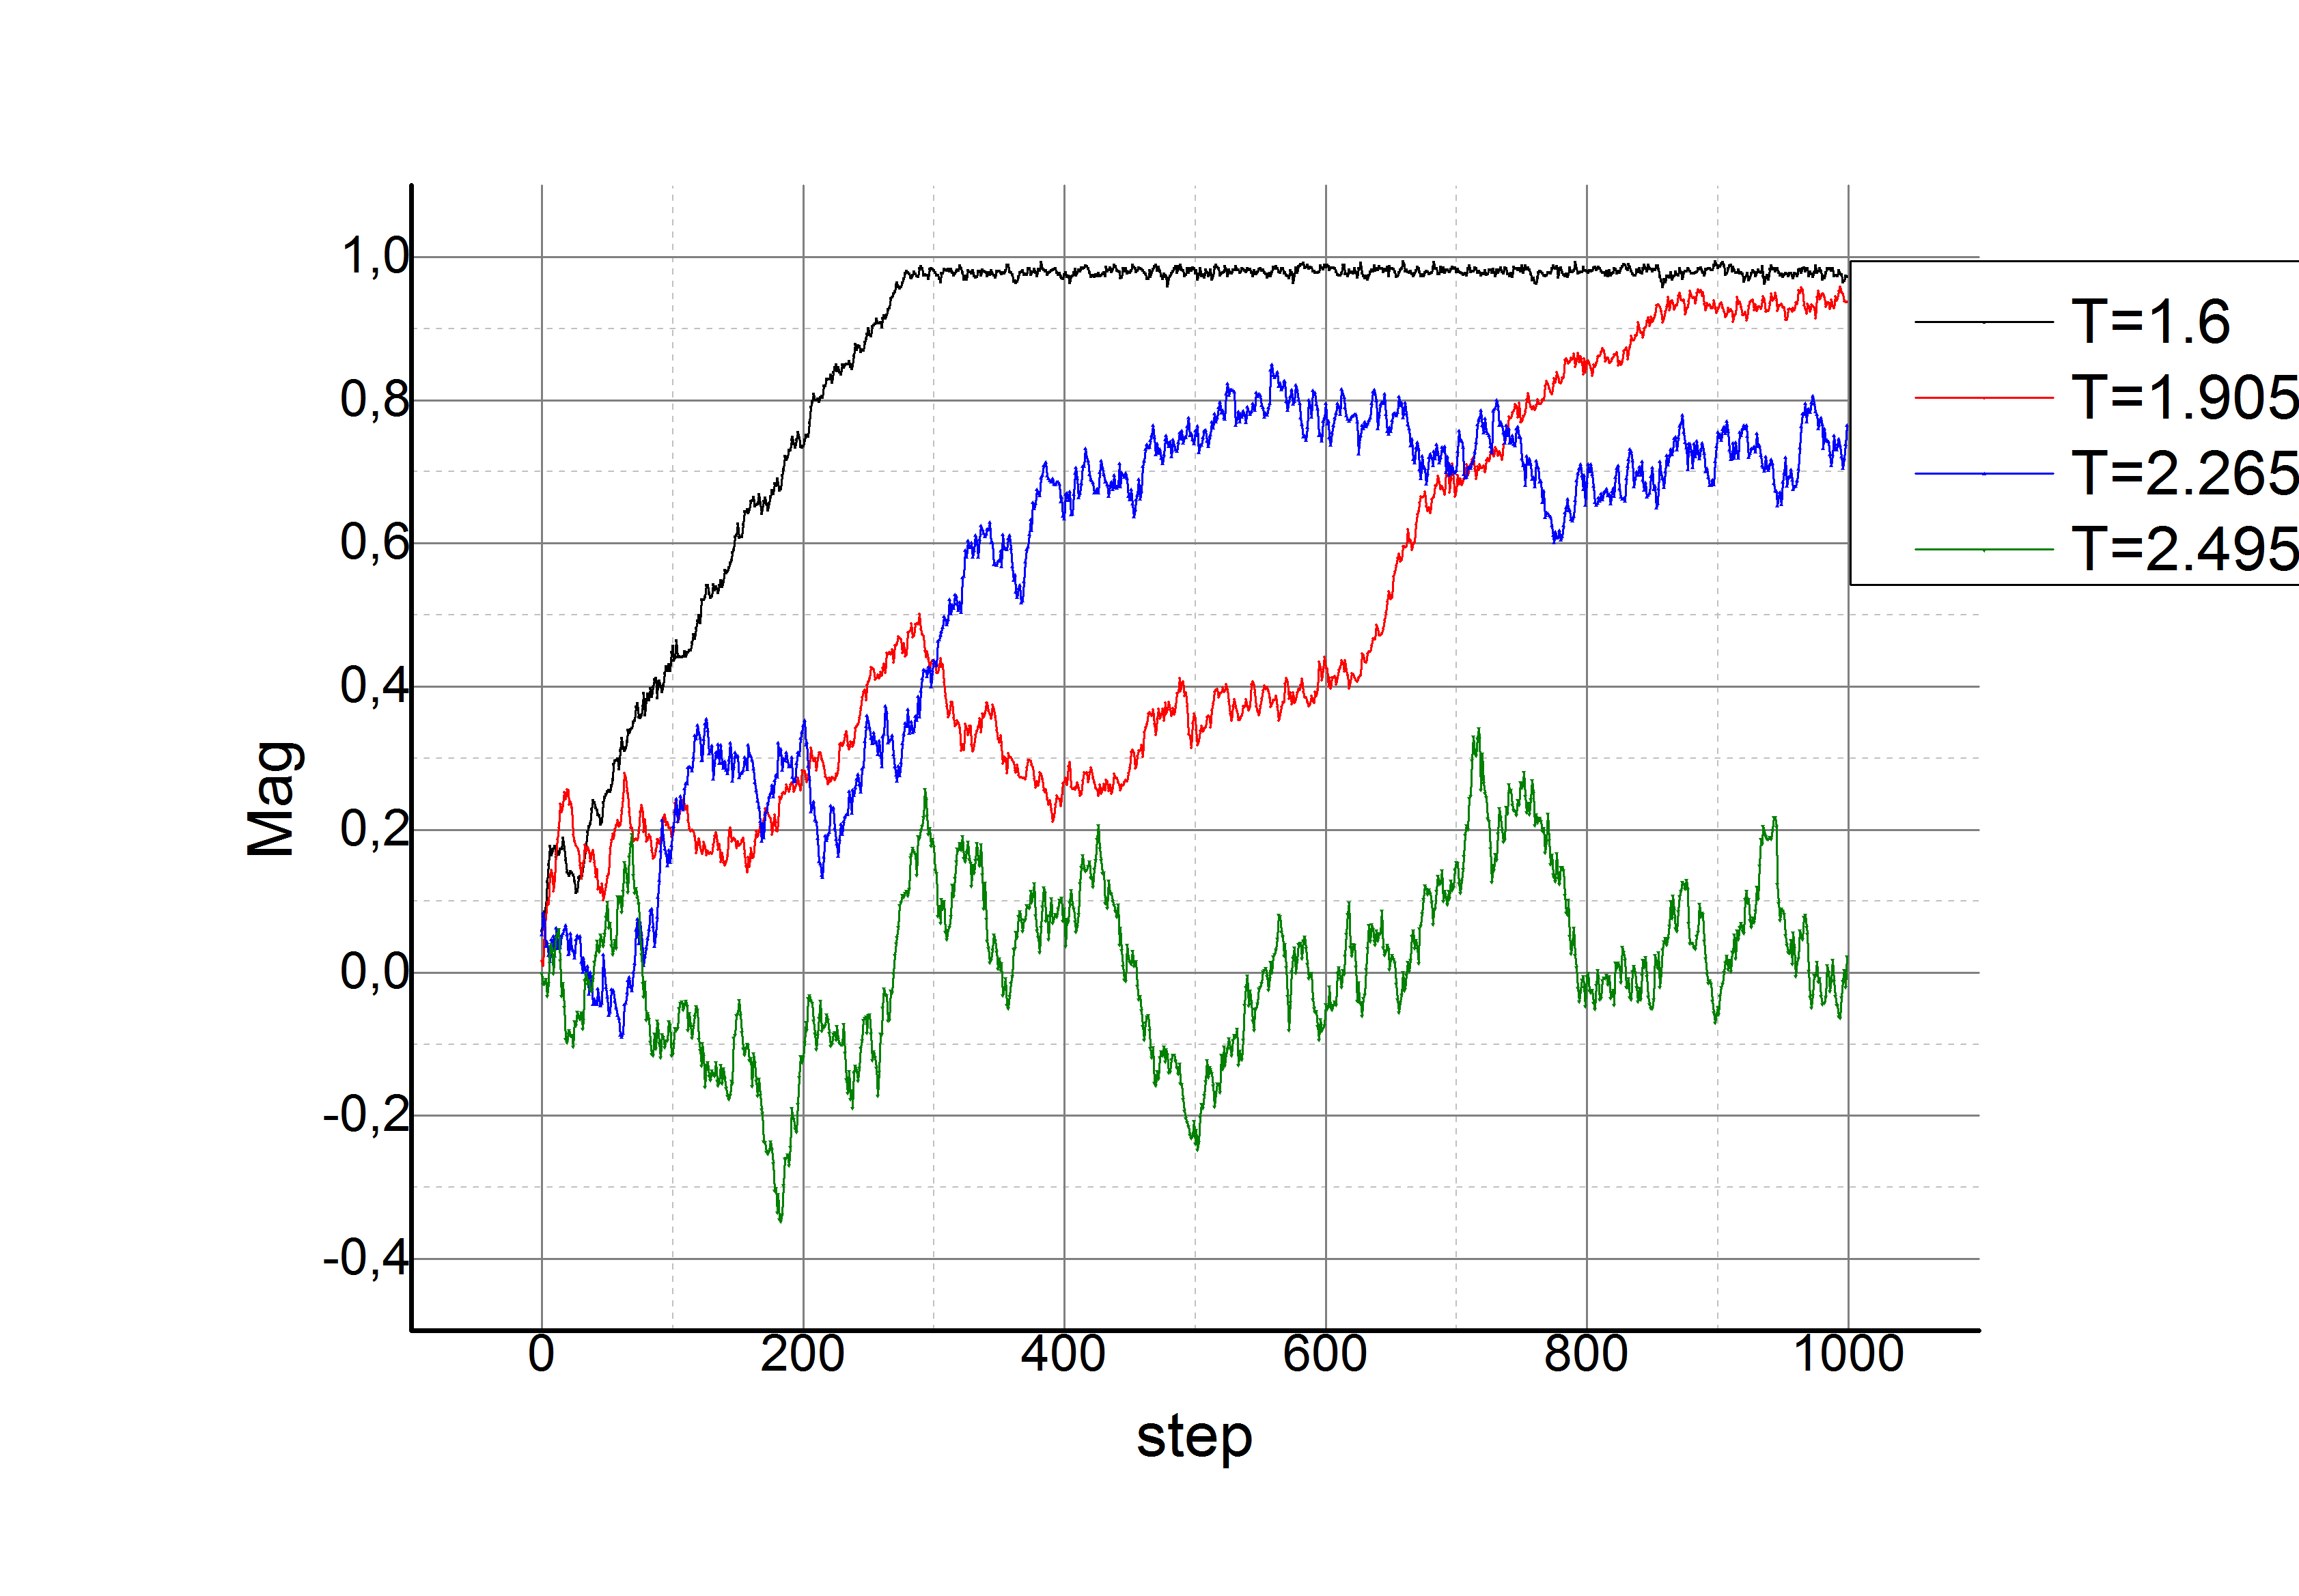
\includegraphics[width=0.47\textwidth]{../Graph_Export/MP2D/m(Steps)_r.jpg}
}	
	\subfigure[positv parallele Startkonfiguration]{
		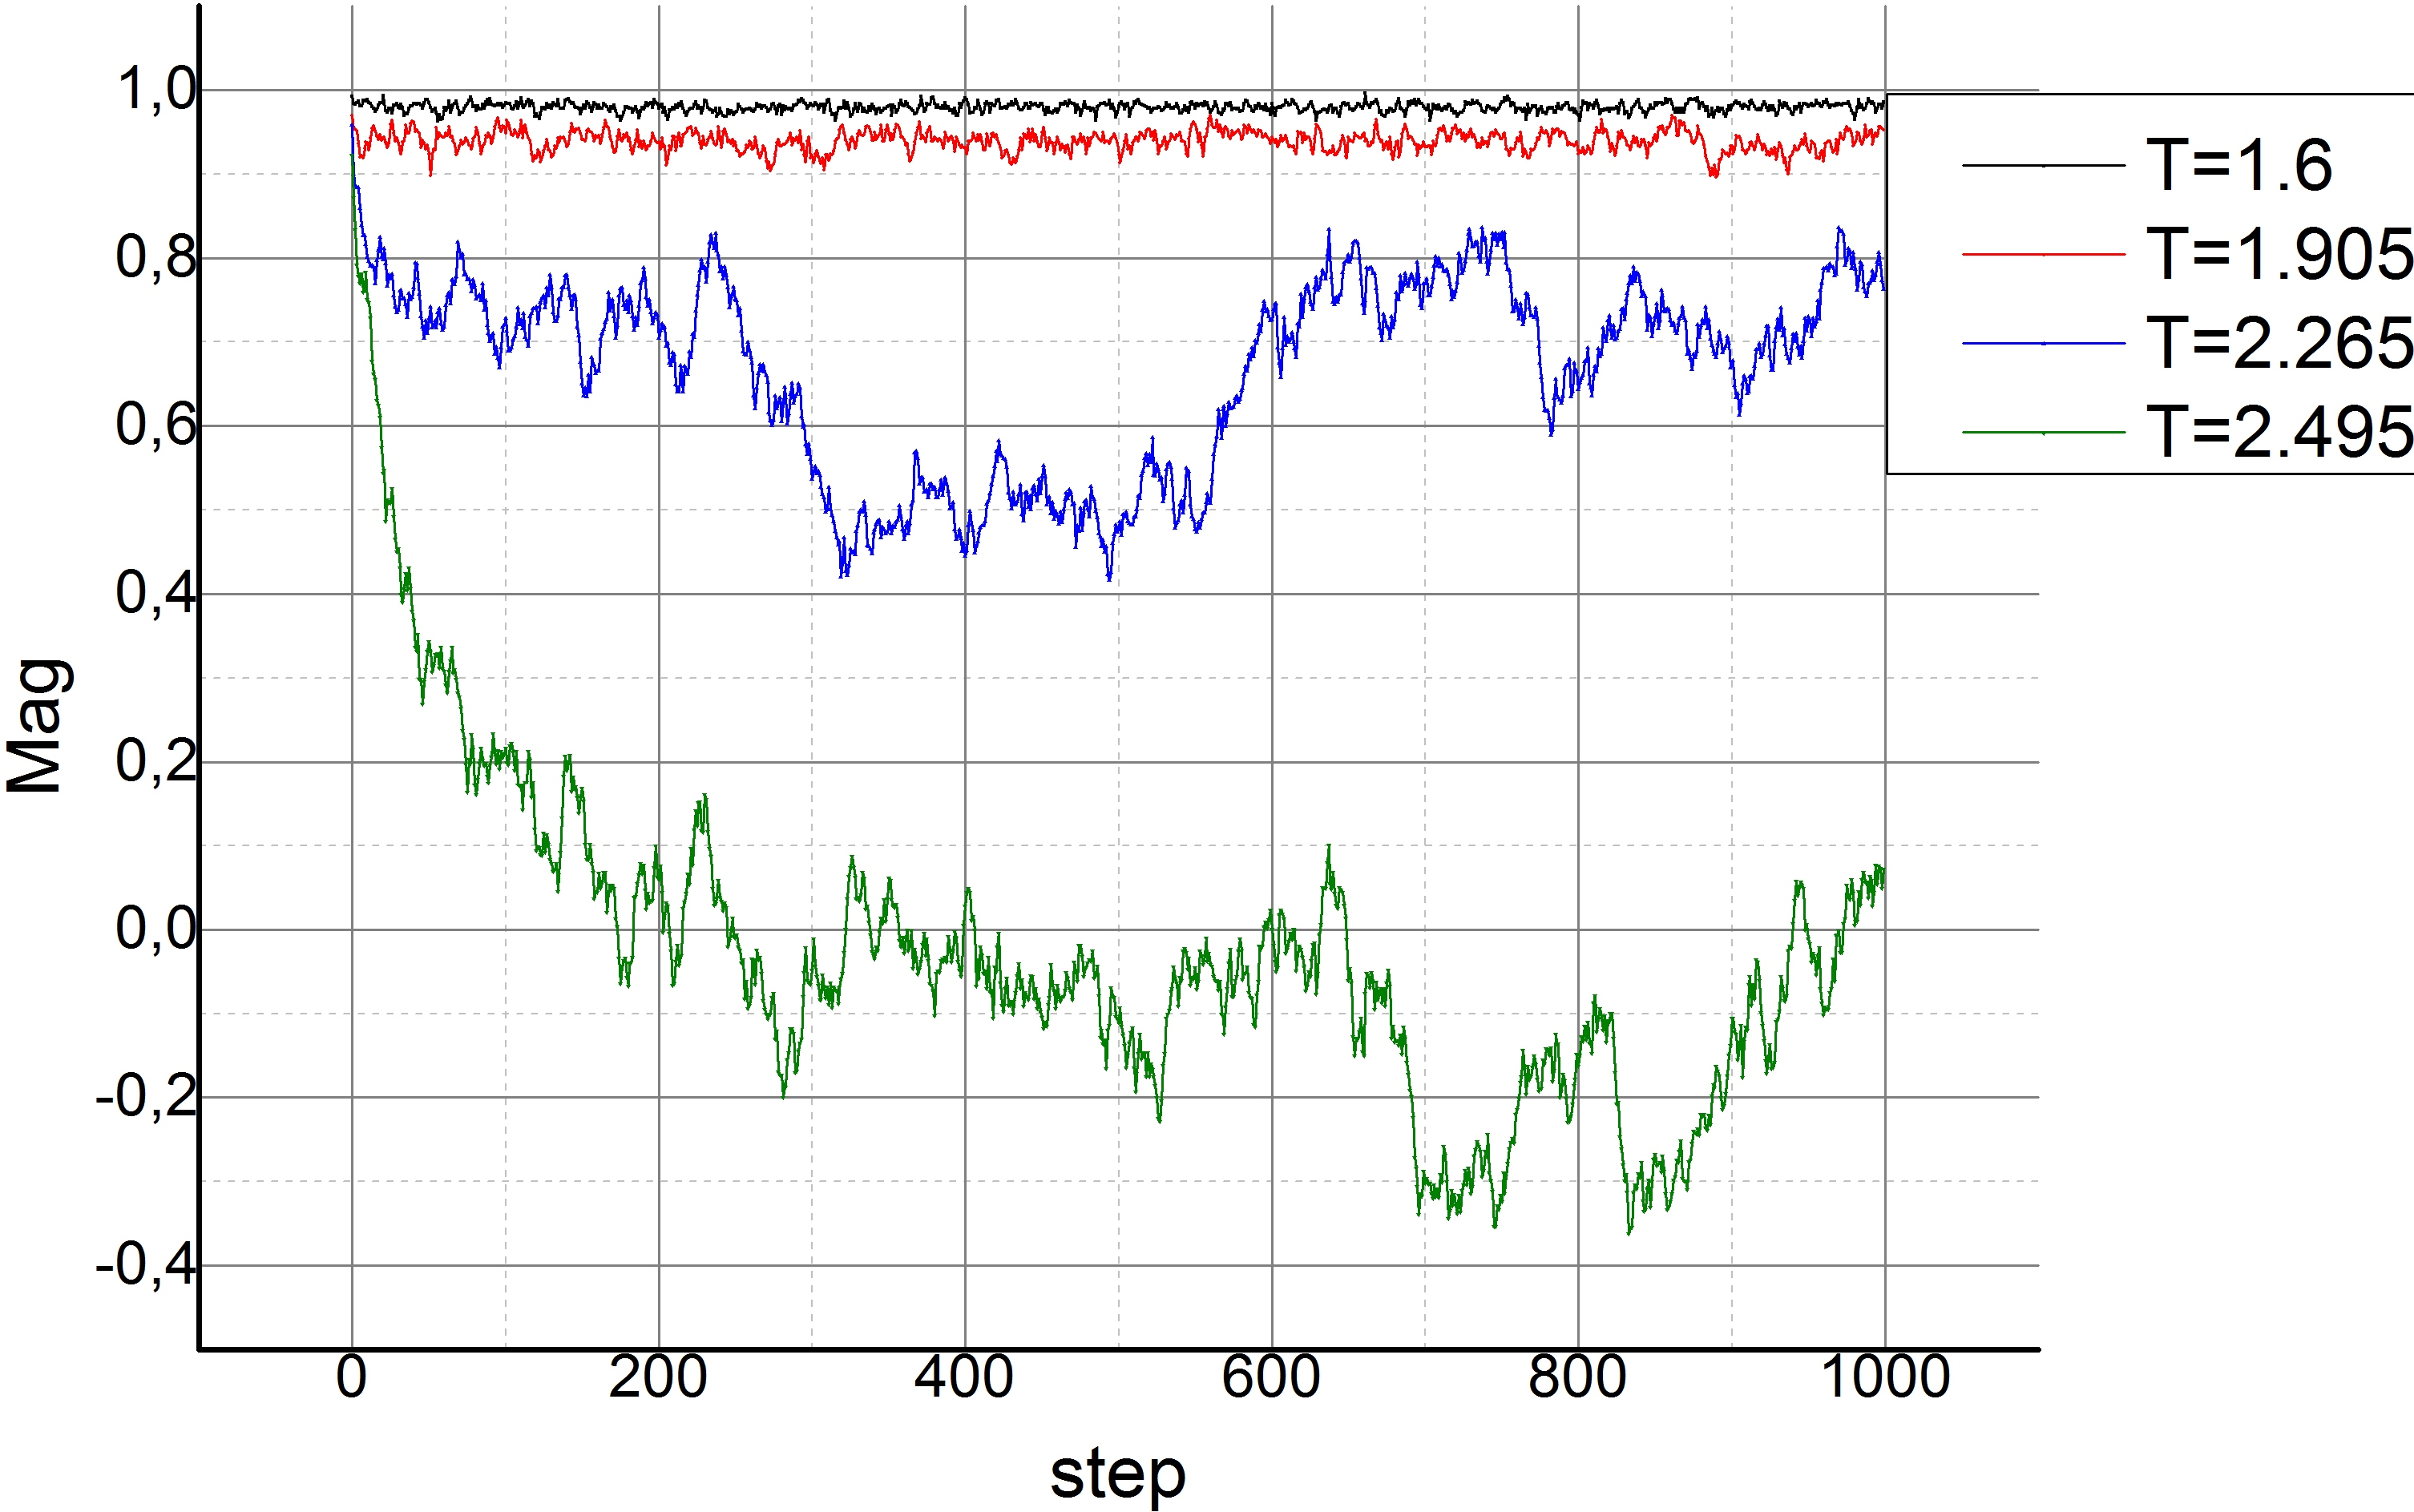
\includegraphics[width=0.47\textwidth]{../Graph_Export/MP2D/m(Steps)_p.jpg}
}		
	\caption{Konvergenzverhalten der Magnetisierung im Metropolisalgorithmus für ein zweidimensionales Gitter}
	\label{mp2dkonv}
\end{figure}

3D

\begin{figure}[H]
	\centering
	\subfigure[zufällige Startkonfiguration]{
		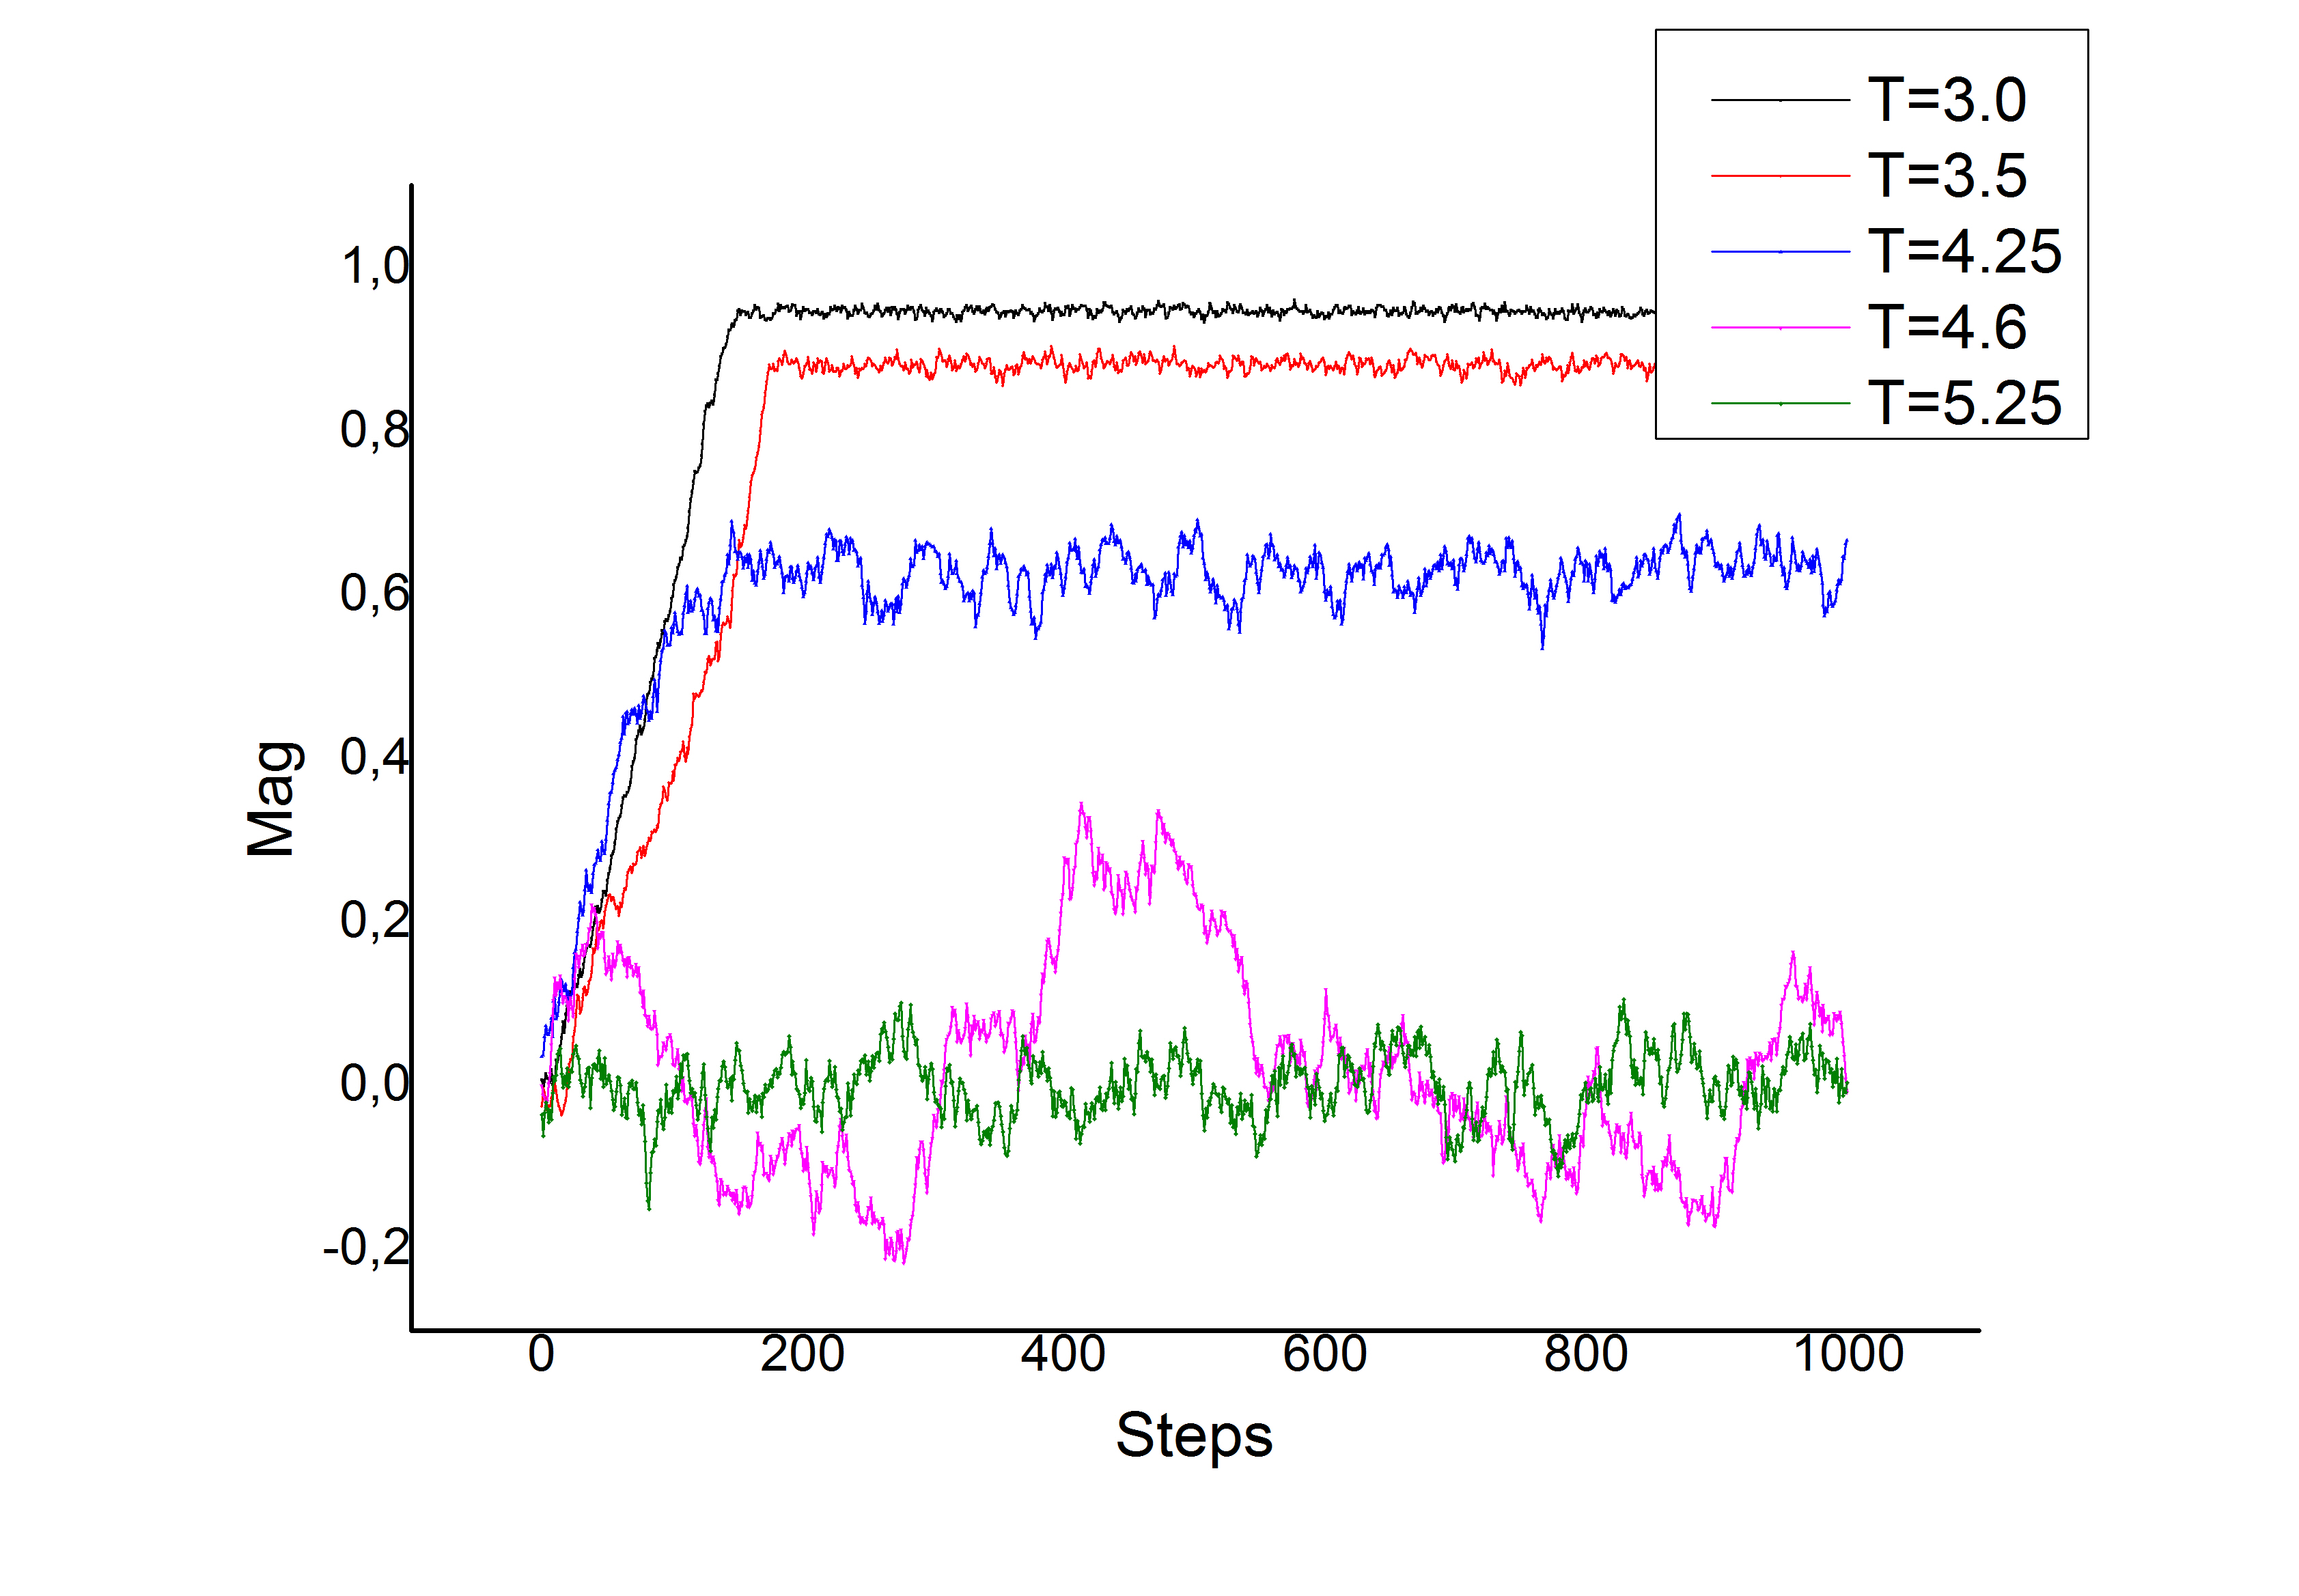
\includegraphics[width=0.47\textwidth]{../Graph_Export/MP3D/m(Steps)_r.jpg}
}	
	\subfigure[positv parallele Startkonfiguration]{
		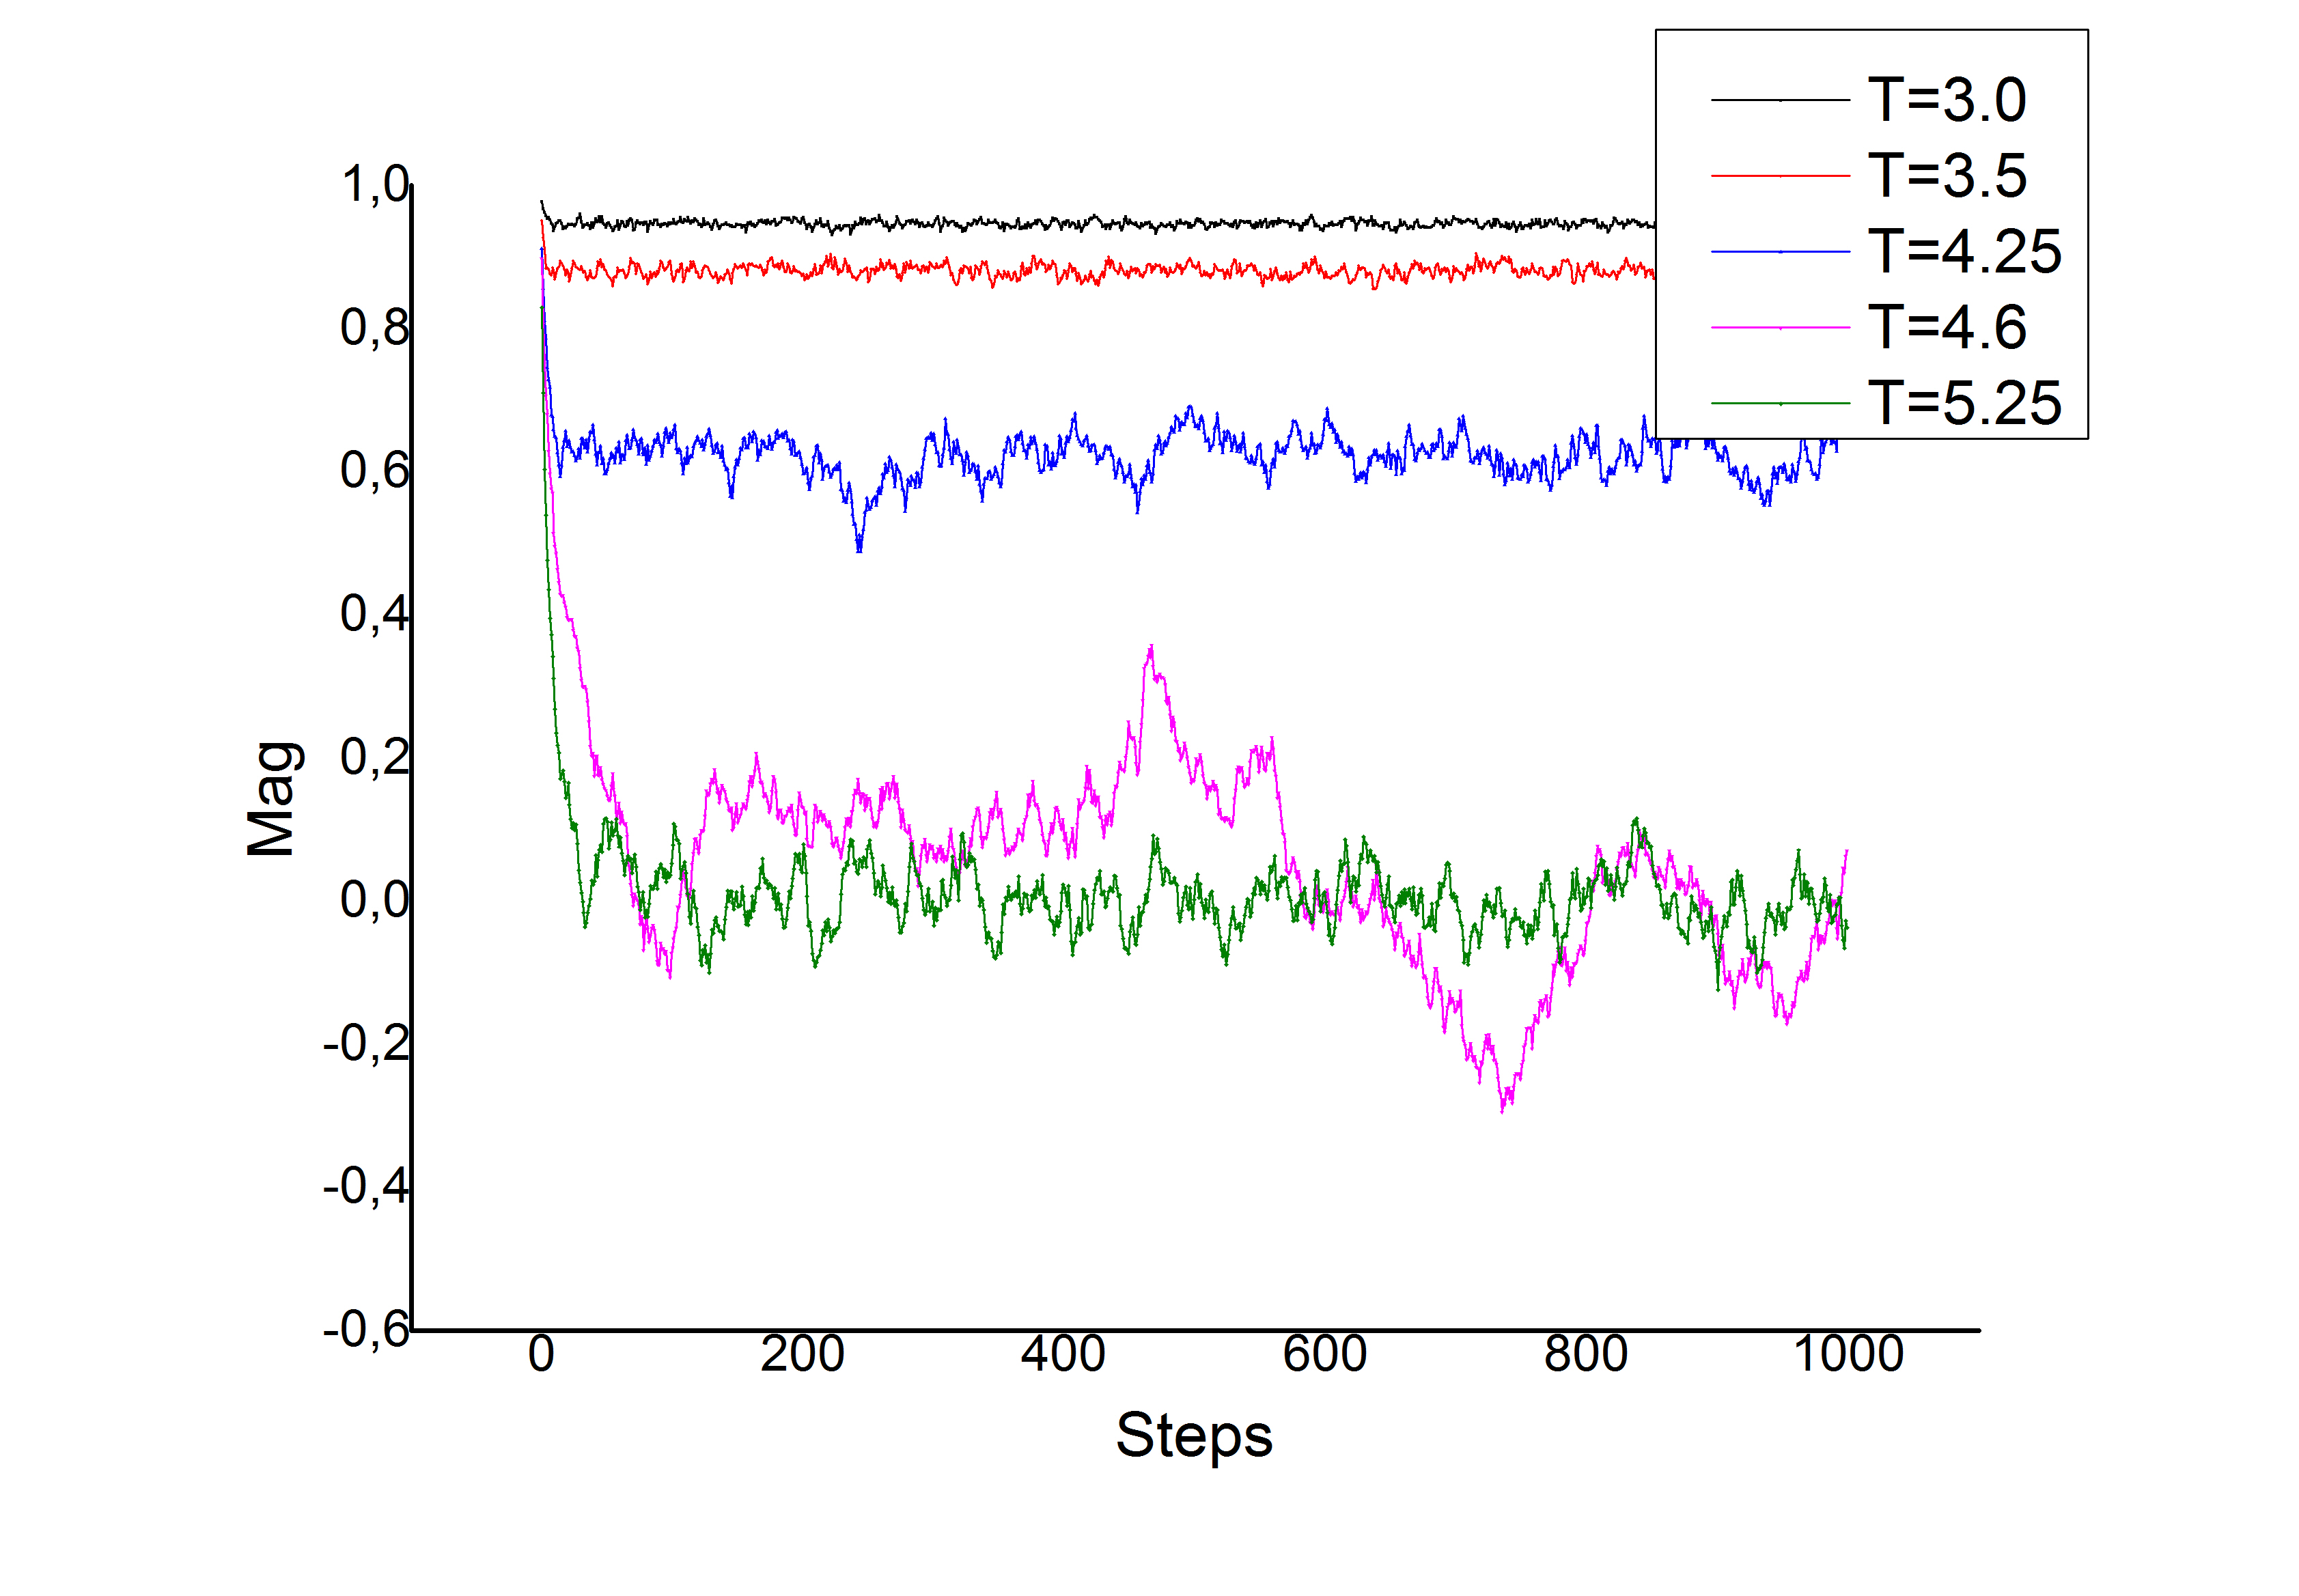
\includegraphics[width=0.47\textwidth]{../Graph_Export/MP3D/m(Steps)_p.jpg}
}		
	\caption{Konvergenzverhalten der Magnetisierung im Metropolisalgorithmus für ein dreidimensionales Gitter}
	\label{mp3dkonv}
\end{figure}

\subsection{Im Detail: Funktion weiterer Parameter}

Außer der Wahl der Gittergröße, der Anzahl an Monte-Carlo-Schritten und der Dimension (2D oder 3D) bietet das Programm noch weitere Parameter, mit denen verschiedene Simulationsmodi gestartet werden können.\\
Um nicht nur den Einfluss der Temperatur, sondern auch den des äußeren Magnetfeldes untersuchen zu können, gibt es die Möglichkeit, die zwischen den verschiedenen Simulationen zu variierende Größe zu wählen. So wird entweder der Tempeartur- oder der Magnetfeldbereich zwischen dem als Parameter angegebenen Start- und Endwert mit einer ebenfalls angegebenen Schrittweite durchlaufen.\\
Möchte man das Schaltverhalten des Systems untersuchen, stellt man mit Hilfe eines Parameters ein, dass bei der Variation des Magnetfeldes nicht bei jeder neuen Feldstärke ein zufälliges neues Gitter erstellt wird, sondern auf dem vorhandenen weitergearbeitet wird. Außerdem wird in diesem Fall der angegebene Bereich nicht nur in eine Richtung durchlaufen, sondern anschließend auch zurück, sodass eine Hysterese erkennbar werden kann.\\
Dazu ist es noch möglich, mit einem vollständig ausgerichteten Gitter zu beginnen, sowie die Cluster-Update-Methode zu verwenden oder nicht und zur Veranschaulichung des Systems, einige Zwischenergebnisse als Dateien zu speichern.
